\input{../header.tex}
\usepackage{tikz}
\usetikzlibrary{arrows.meta}
\usetikzlibrary{decorations.pathreplacing}
\usepackage[dvipsnames]{xcolor}
\usetikzlibrary{trees}
\usepackage{tcolorbox}

\usepackage{listings}

\hypersetup{
    colorlinks=true,
    linkcolor=blue,
    filecolor=magenta,      
    urlcolor=blue,
    pdfpagemode=FullScreen,
    }

\usepackage{array}
\newcolumntype{C}[1]{>{\centering\let\newline\\\arraybackslash\hspace{0pt}}m{#1}}
\lstset{upquote=true,basicstyle=\fontencoding{T1}\selectfont\ttfamily}
\def\x{1}
\def\y{1}
\begin{document}

% Change the following values to true to show the solutions or/and the hints
\ShowSolutiontrue
\ShowConseiltrue
\ShowWarningtrue
\titre
\cours{Programmation de base}

Le but de cette séance est d'aborder des notions de base en programmation. Au terme de cette séance, vous serez capable de: \\

\begin{itemize}
    \item Comprendre les différentes représentations de nombres.
	\item Définir des variables et comprendre les types de variables existants.
	\item Utiliser des notions d'algèbre booléenne.
    \item Ecrire des branchements conditionnels.\\
\end{itemize} 

Les langages qui seront utilisés pour cette séance sont Java et Python. Assurez-vous d'avoir bien installé Intellij. Si vous rencontrez des difficultés, n'hésitez pas à vous référer au guide suivant: \href{https://moodle.unil.ch/pluginfile.php/3532600/mod_resource/content/9/prerequisite_macos.pdf}{tutoriel d'installation des outils (MacOS) et prise en main de l'environnement de travail} ou \href{https://moodle.unil.ch/pluginfile.php/3691183/mod_resource/content/9/prerequisite_win.pdf}{tutoriel d'installation des outils (Windows)}.

\section{Input / Output}

\begin{Exercice}[5 minutes] \textbf{Output (Java ou Python)}\\
   Créez une variable \textit{nom} (str) contenant votre nom, et une autre \textit{prenom} (str) contenant votre prénom puis affichez : "Bonjour, \textit{prenom nom}". \\
   
    \begin{conseil}
        Utilisez la fonction \lstinline{print()} de Python et \lstinline{System.out.println()} de Java. 
        
    \end{conseil}
    \begin{solution}
    
    \textbf{Python:} 
    \lstinputlisting{solutions/question1.py}
    
    \textbf{\\Java:} 
    \lstinputlisting{solutions/Question1.java}  
    \end{solution}   
\end{Exercice}

\begin{Exercice}[5 minutes] \textbf{Input (Java ou Python)}\\
   En vous référant à l'exercice précédent (\textbf{Output (Java ou Python)}), demandez à l'utilisateur d'entrer son nom et son prénom via la fonction \lstinline{input()} au lieu d'initialiser vous-même les variables. \\
   
    \begin{conseil}
       Utilisez la fonction \lstinline{input()} en Python, la classe \lstinline{Scanner()} en Java (n'oubliez pas d'ajouter \lstinline{import java.util.Scanner;}) tout au début de votre code. 
        
    \end{conseil}
    \begin{solution}
    
    \textbf{Python:} 
    \lstinputlisting{solutions/question2.py}
    
    \textbf{\\Java:}
    \lstinputlisting{solutions/Question2.java}  
       
        
    \end{solution}   
\end{Exercice}


\section{Représentation de nombres entiers}

\begin{Exercice}[5 minutes] \textbf{Entiers non signés}\\
	Sur 8 bits, convertir 113$_{(10)}$ en base binaire.
   
    \begin{conseil}
		Faire un tableau comme présenté dans la diapositive 15 du cours (programmation de base). Essayer de décomposer le nombre en une somme de puissances de 2.
    \end{conseil}
    
    \begin{solution}
        Méthode 1: Utiliser la division par 2 comme vu dans la première séance d'exercices.\\

        \begin{center}
        \begin{minipage}{0.3\textwidth}
    \centering

     \resizebox{\textwidth}{!}{%
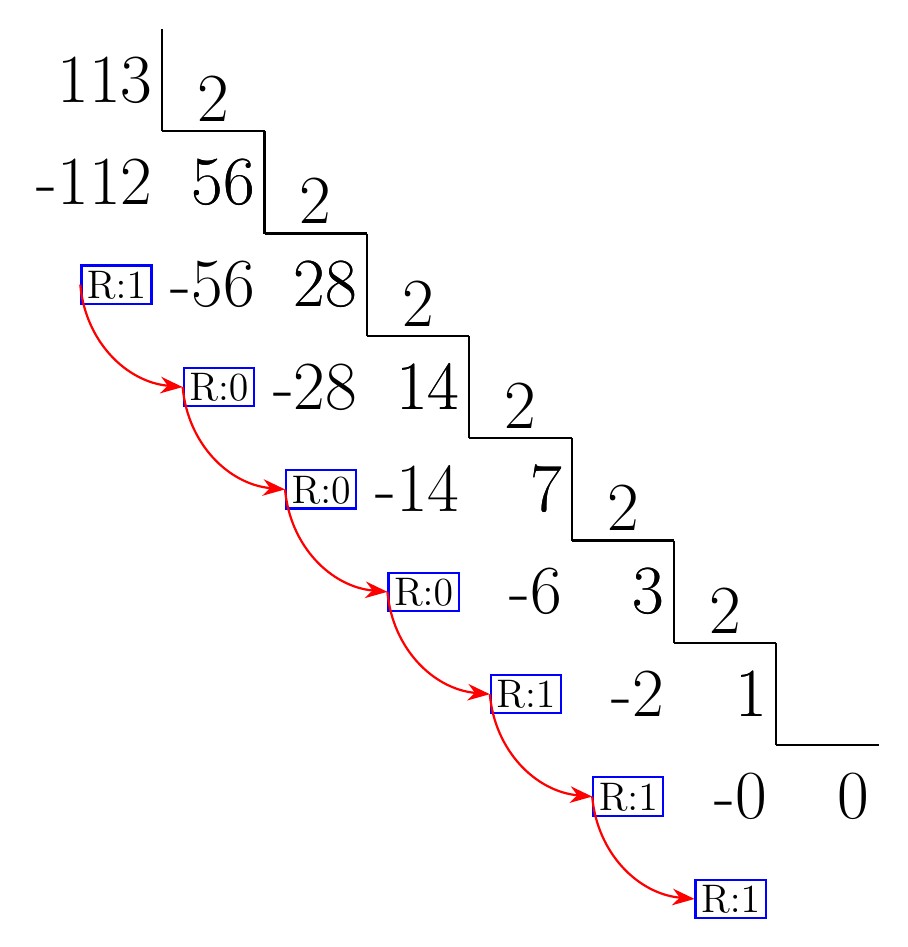
\begin{tikzpicture}[scale=1.3]
        % Ladder pattern: vertical down, horizontal right, vertical down, horizontal right, etc.
    \draw[thick] (0,4) -- (0,3);        % vertical down
    \node[left] at (0,3.5) {\Huge 113};)
    \node[left] at (0,2.5) {\Huge -112};)
    \node[right, draw=blue, thick, inner sep=2pt] at (0.2-\x,2.5-\y) {\Large R:1};)
    \draw[thick] (0,3) -- (1,3);        % horizontal right
    \node[above] at (0.5,3) {\Huge 2};
    \node[left] at (1,2.5) {\Huge 56};)
    \draw[thick] (1,3) -- (1,2);        % vertical down
    \node[left] at (1,2.5) {\Huge 56};)
    \node[left] at (1,1.5) {\Huge -56};)
    \node[right, draw=blue, thick, inner sep=2pt] at (1.2-\x,1.5-\y) {\Large R:0};)
    \draw[thick] (1,2) -- (2,2);        % horizontal right
    \node[above] at (1.5,2) {\Huge 2};
    \node[left] at (2,1.5) {\Huge 28};)
    \draw[thick] (2,2) -- (2,1);        % vertical down
    \node[left] at (2,1.5) {\Huge 28};)
    \node[left] at (2,0.5) {\Huge -28};)
    \node[right, draw=blue, thick, inner sep=2pt] at (2.2-\x,0.5-\y) {\Large R:0};)
    \draw[thick] (2,1) -- (3,1);        % horizontal right
    \node[above] at (2.5,1) {\Huge 2};
    \node[left] at (3,0.5) {\Huge 14};)
    \draw[thick] (3,1) -- (3,0);        % vertical down
    \node[left] at (3,0.5) {\Huge 14};)
    \node[left] at (3,-0.5) {\Huge -14};)
    \node[right, draw=blue, thick, inner sep=2pt] at (3.2-\x,-0.5-\y) {\Large R:0};)
    \draw[thick] (3,0) -- (4,0);        % horizontal right
    \node[above] at (3.5,0) {\Huge 2};
    \node[left] at (4,-0.5) {\Huge 7};)
    \draw[thick] (4,0) -- (4,-1);        % vertical down
    \node[left] at (4,-0.5) {\Huge 7};)
    \node[left] at (4,-1.5) {\Huge -6};)
    \node[right, draw=blue, thick, inner sep=2pt] at (4.2-\x,-1.5-\y) {\Large R:1};)
    \draw[thick] (4,-1) -- (5,-1);        % horizontal right
    \node[above] at (4.5,-1) {\Huge 2};
    \node[left] at (5,-1.5) {\Huge 3};)
    \draw[thick] (5,-1) -- (5,-2);        % vertical down
    \node[left] at (5,-1.5) {\Huge 3};)
    \node[left] at (5,-2.5) {\Huge -2};)
    \node[right, draw=blue, thick, inner sep=2pt] at (5.2-\x,-2.5-\y) {\Large R:1};)
    \draw[thick] (5,-2) -- (6,-2);        % horizontal right
    \node[above] at (5.5,-2) {\Huge 2};
    \node[left] at (6,-2.5) {\Huge 1};)
    \draw[thick] (6,-2) -- (6,-3);        % vertical down
    \node[left] at (6,-2.5) {\Huge 1};)
    \node[left] at (6,-3.5) {\Huge -0};)
    \node[right, draw=blue, thick, inner sep=2pt] at (6.2-\x,-3.5-\y) {\Large R:1};)
    \node[left] at (7,-3.5) {\Huge 0};
    \draw[thick] (6,-3) -- (7,-3);
    
    % Red curves connecting all blue border nodes
    % Define the positions of the blue border nodes
    \coordinate (node1) at (0.2-\x,2.5-\y);
    \coordinate (node2) at (1.2-\x,1.5-\y);
    \coordinate (node3) at (2.2-\x,0.5-\y);
    \coordinate (node4) at (3.2-\x,-0.5-\y);
    \coordinate (node5) at (4.2-\x,-1.5-\y);
    \coordinate (node6) at (5.2-\x,-2.5-\y);
    \coordinate (node7) at (6.2-\x,-3.5-\y);
    
    % Connect nodes with red curves
    \draw[red, thick, bend right=40, -{Stealth[length=8pt,width=6pt]}] (node1) to (node2);
    \draw[red, thick, bend right=40, -{Stealth[length=8pt,width=6pt]}] (node2) to (node3);
    \draw[red, thick, bend right=40, -{Stealth[length=8pt,width=6pt]}] (node3) to (node4);
    \draw[red, thick, bend right=40, -{Stealth[length=8pt,width=6pt]}] (node4) to (node5);
    \draw[red, thick, bend right=40, -{Stealth[length=8pt,width=6pt]}] (node5) to (node6);
    \draw[red, thick, bend right=40, -{Stealth[length=8pt,width=6pt]}] (node6) to (node7);
    
\end{tikzpicture}
     }
\end{minipage}
        \end{center}
        
        Méthode 2 : Utiliser les puissances de 2 pour décomposer le nombre (vu également dans la première séance d'exercices).
        
        113 = 64 + 32 + 16 + 1 = 1 * $2^6$ + 1 * $2^5$ + 1* $2^4$ + 1 * $2^0$ \\
        
        \begin{tabular}{| p{1cm} | p{1cm} | p{1cm} | p{1cm} | p{1cm} | p{1cm} | p{1cm} | p{1cm} | p{1cm} |} 
            \hline
	      	$2^7$ & $2^6$ & $2^5$ & $2^4$ & $2^3$ & $2^2$ & $2^1$ & $2^0$ \\ [0.5ex]
	    	\hline
            128 & 64 & 32 & 16 & 8 & 4 & 2 & 1 \\ [0.5ex] 
            \hline
            0 & 1 & 1 & 1 & 0 & 0 & 0 & 1 \\ [0.5ex] 
            \hline
        \end{tabular} \\
        
        On obtient donc 01110001$_{(2)}$ \\
    \end{solution}
\end{Exercice}

\begin{Exercice}[5 minutes] \textbf{Entiers signés négatifs}\\
    En utilisant le résultat de la question précédente, convertir sur 8 bits -113$_{(10)}$ en base binaire. Utiliser la représentation \textbf{signée} à la diapositive 15 du cours (et non le complément à 1 ou 2). \\

    \begin{conseil}
        \begin{itemize}
        	\item Il faut prendre la représentation sur 7 bits d'un nombre entier non signé.
        	\item On rajoute un 8ème bit qui sera le signe.
        	\item Le premier bit à gauche vaut 0 pour un nombre positif et 1 pour un nombre négatif.
        \end{itemize} 
    \end{conseil}
    
    \begin{solution}
         113$_{(10)}$ = 01110001$_{(2)}$ \\
         
         En changeant le premier bit à 1 pour faire passer le nombre en nombre négatif on obtient : \\
         
         -113$_{(10)}$ = 11110001$_{(2)}$ \\
    \end{solution}
\end{Exercice}

\begin{Exercice}[5 minutes] \textbf{Complément à 1}\\
    Écrire le complément à 1 de -113$_{(10)}$ sur 8 bits. \\

	Quelle est la différence entre cette méthode et la précédente ?

    \begin{conseil}
        \begin{itemize}
        	\item L'opposé de 0 en binaire est 1 et inversément.
        	\item Pour étudier la différence, il faut regarder les différentes manières d'exprimer -0 en binaire (se référer à la diapositive 16 du cours).
        \end{itemize} 
    \end{conseil}
    
    \begin{solution}
    	113$_{(10)}$ = 01110001$_{(2)}$ \\
    	
        \begin{tabular}{| p{1cm} | p{1cm} | p{1cm} | p{1cm} | p{1cm} | p{1cm} | p{1cm} | p{1cm} | p{1cm} |} 
            \hline
            0 & 1 & 1 & 1 & 0 & 0 & 0 & 1 \\ [0.5ex] 
            \hline
            not & not & not & not & not & not & not & not \\ [0.5ex]
            \hline
            1 & 0 & 0 & 0 & 1 & 1 & 1 & 0 \\ [0.5ex]
            \hline
        \end{tabular} \\
        
        avec cette méthode, -113$_{(10)}$ = 10001110$_{(2)}$ \\
        
        L'intervalle de cette méthode ne change pas par rapport à la précédente. Par contre, l'expression de -0 sera différente.\\
        
        Signé: -0$_{(10)}$ = 10000000$_{(2)}$ \\
        
        Complément à 1: -0$_{(10)}$ = 11111111$_{(2)}$ \\
        
        Les deux ont le même intervalle: [-127$_{(10)}$,+127$_{(10)}$] \\
        
    \end{solution}
\end{Exercice}

\begin{Exercice}[5 minutes] \textbf{Complément à 2}\\
    Quelle est la représentation du complément à 2 (two complement) de -113$_{(10)}$ sur 8 bits et quelle est l'utilité de cette représentation ? \\

    \begin{conseil}
    
    Exemple du cours avec 87$_{(10)}$ \\
    
    87$_{(10)}$ = 01010111$_{(2)}$ \\
    
         \begin{tabular}{| p{1cm} | p{1cm} | p{1cm} | p{1cm} | p{1cm} | p{1cm} | p{1cm} | p{1cm} | p{1cm} |} 
            \hline
            a & 0 & 1 & 0 & 1 & 0 & 1 & 1 & 1 \\ [0.5ex] 
            \hline
            b & 1 & 0 & 1 & 0 & 1 & 0 & 0 & 0 \\ [0.5ex]
            \hline
            c & 1 & 0 & 1 & 0 & 1 & 0 & 0 & 1 \\ [0.5ex]
            \hline
        \end{tabular} \\
        
        a : convertir le nombre en binaire \\
        
        b : inverser tous les bits (en utilisant \textbf{not}) \\
        
        c : rajouter 1 à b pour obtenir le complément à 2 \\
        
        On obtient donc -87$_{(10)}$ = 10101001$_{(2)}$ \\
    \end{conseil}
    
    \begin{solution}
    	Ici, il suffit donc d'ajouter 1 au complément à 1 de -113$_{(10)}$ \\
    	
    	On obtient donc 10001111$_{(2)}$ \\
    	
    	Concernant l'intervalle, il est changé, étant donné qu'il n'existe plus qu'une seule représentation possible pour -0$_{(10)}$. \\
    	
    	Le nouvel intervalle est donc [-128$_{(10)}$,+127$_{(10)}$]
        
    \end{solution}
\end{Exercice}

\begin{Exercice}[10 minutes] \textbf{Floating point}\\
    
    Voici la représentation en binaire d'un nombre à virgule flottante: \\
    
     \begin{tabular}{| p{1cm} | p{3cm} | p{9.5cm} | p{1cm} | p{1cm} | p{1cm} | p{1cm} | p{1cm} | p{1cm} |} 
            \hline
            signe & exposant & mantisse \\ [0.5ex] 
            \hline
            0 & 10110101 & 01000001000000000000001 \\ [0.5ex]
            \hline
	\end{tabular}
	\\
    
    Que vaut cette représentation en base 10 ? Utiliser la représentation des floating points (avec un biais de 127). Arrondir les résultats intermédiaires et la valeur finale au 3ème chiffre significatif après la virgule. \\
	
    \begin{conseil}
    
    \begin{itemize}
    	\item Se référer à la diapositive 23 du cours pour plus de détails.
    	\item Poser chaque calcul, et ensuite tout fusionner avec la formule.
    	\item L'exposant et la mantisse sont des entiers positifs, donc non signés.
    	\item Pour vérifier votre résultat, vous pouvez utiliser l'outil suivant: \url{https://www.h-schmidt.net/FloatConverter/IEEE754.html}
    \end{itemize}
    
    \end{conseil}
    
    \begin{solution}
        \begin{itemize}
        	\item Signe du nombre : $(-1)^{signe}$ = $(-1)^0$ = 1
        	\item Exposant en base 10 : 10110101$_{(2)}$ = 181$_{(10)}$
        	\item Pour obtenir l'exposant, il faut encore lui appliquer le biais, il faut soustraire 127 à notre résultat. Ici on aura $2^{(181-127)}$ = $2^{54}$
        	\item Mantisse : 01000001000000000000001$_{(2)}$ = 1 + 1*$2^{-2}$ + 1*$2^{-8}$ + 1*$2^{-23}$ = 1.254$_{(10)}$
        	\item Valeur = Signe * Mantisse * $2^{exposant-127}$ = 1 * 1.254 * $2^{54}$ = 2.259 * $10^{16}$
        \end{itemize}
    \end{solution}
\end{Exercice}

\section{Typage}

Le but de cette partie des travaux pratiques est de comprendre les notions de typage statique et dynamique, ainsi que leur impact sur l’exécution et la gestion des erreurs. \\

\begin{Exercice}[5 minutes]  \textbf{Les types de variables}\\
    
    Quelles sont les principaux types de variables (donnez en 3), comment les déclareriez-vous en Python et en Java ? \\

    \begin{conseil}
    
        Se référer aux diapositives du cours ou à la documentation officielle des langages de programmation.
        
    \end{conseil}
    \begin{solution}
    
        Les principaux types de variables sont les suivants : \lstinline{Integer (int), Float, String (str), Boolean (bool)}.\\

		En Python :    
        
    	\lstinputlisting{solutions/question8.py} 
    	
    	
    	En Java : 
    	
    	\lstinputlisting{solutions/Question8.java} 
    	
    	Il existe d'autres types de variable, comme par exemple les \lstinline{double}.
 
    \end{solution}
\end{Exercice}


\begin{Exercice}[10 minutes]  \textbf{Typage statique et dynamique}\\
    
    Parmi ces différents programmes, lesquels pourront être exécutés sans problème et lesquels lèveront des erreurs? Dans le cas où ils génèreraient des erreurs, expliquez la raison de ces erreurs.\\
    
    \textbf{Java :}
    
    \lstinputlisting{code/Question9.java} 
    
    \textbf{Python :}
    
    \lstinputlisting{code/question9.py} 
    

    \begin{conseil}
    
        En Java, le type est statique, ce qui signifie qu'à partir du moment où vous créez une variable, un type va lui être attribué (par vous ou par le code en lui-même par déduction). Ce type ne pourra pas être changé, et si vous tentez de le faire (en lui attribuant une valeur d'un autre type par exemple), une erreur sera levée. \\

En Python, le typage est dynamique, il est donc tout à fait possible de changer le type d'une variable sans déclencher d'erreur. \\

    \end{conseil}

    \begin{Example}{\faTriangleExclamation \quad Erreurs fréquentes}
        Au cas où vous exécuteriez les programmes 2, 4 et 5 et rencontriez l'erreur suivante: \lstinline{Exception in thread "main" java.lang.UnsupportedClassVersionError: ... has been compiled by a more recent version of the Java Runtime (class file version 54.0), this version of the Java Runtime only recognizes class file versions up to 52.0}, suivez les étapes ci-dessous:
        \begin{enumerate}
            \item Mettez à jour votre JDK en téléchargeant la version adéquate via le lien suivant: \url{https://www.oracle.com/java/technologies/downloads/}.
            \item Une fois votre JDK installé, redémarrez IntelliJ
            \item Dans la barre de menus, cliquez sur \textbf{\faEllipsisVertical \ $>$ \ Edit...}.
            \item Dans la fenêtre qui apparaitra (capture ci-dessous), sélectionnez la version du JRE la plus récente.
        \end{enumerate}
        
    \end{Example}
    \begin{figure}[h]
        \centering
        
\includegraphics[width=1\textwidth]{img/jre.png}
        \caption{Fenêtre de configuration de l'environnement de développement Java.}
    \end{figure}
    \begin{solution}

        \textbf{En Java}        
        \begin{itemize}
        	\item Programme 1 : OK
        	\item Programme 2 : Ce code ne fonctionnera pas car on essaye de changer le type de la variable\_2, ce qui est impossible avec un typage statique comme en java. Ici le type de la variable est ``déduit'' lors de l'exécution du programme.
        	\item Programme 3 : Tout comme le programme précédent, ce code ne fonctionnera pas car on essaye de changer le type de la variable\_2, ce qui est impossible avec un typage statique comme en java.
        	\item Programme 4 : Ce code ne fonctionnera pas car on essaye de changer le type de la variable\_1, ce qui est impossible avec un typage statique comme en java. Ici le type de la variable est ``déduit'' lors de l'exécution du programme.
        	\item Programme 5 : OK
        	\item Programme 6 : Ce code ne fonctionnera pas car on essaye de changer le type de la variable\_1, ce qui est impossible avec un typage statique comme en java. \\
        \end{itemize}
        
        \textbf{En Python}
        
        \begin{itemize}
        	\item Programme 7 : OK
        	\item Programme 8 : OK
        \end{itemize}
        
        
    \end{solution}
\end{Exercice}


\section{Opérateurs et conditions Booléennes}
Le principe d'une valeur booléenne est qu'elle 
ne puisse contenir que 2 valeurs possibles, soit 
\lstinline{True}, soit \lstinline{False}. Il est possible 
de les définir en leur associant une 
de ces valeurs d'emblée ou de les obtenir 
en effectuant une opération booléenne comme par exemple une comparaison. 
Pour ce faire, il faut utiliser des opérateurs booléens. 
Voici les plus utilisés : $=$ (est égal), $!=$ (n'est pas égal), 
$<$ (est strictement plus petit), 
$\leq$ (est plus petit ou égal), $>$ (est strictement plus grand),
 $\geq$ (est plus grand ou égal). Si la condition est satisfaite, on obtiendra \lstinline{True}, si elle ne l'est pas, on obtiendra \lstinline{False}. L'utilisation de l'opérateur \lstinline{not} inversera le résultat.\\

\begin{Exercice}[7 minutes]
\begin{enumerate}
    \item 
 Démontrez l'équivalence suivante:
\begin{align*}
   (\neg p \vee q) \wedge (p \vee \neg q) \Leftrightarrow (p \wedge q) \vee (\neg p \wedge \neg q)
\end{align*}
\begin{conseil}
	Utilisez la table des règles présentées à la diapositive 31 du cours pour déduire cette équivalence. 
\end{conseil}
\item Re-faire cet exercice en utilisant les tables de vérité.
\end{enumerate}
\begin{solution}
   \begin{align*}
   & (\neg p \vee q) \wedge (p \vee \neg q) &\Leftrightarrow   \\
   & ((\neg p \vee q) \wedge p) \vee  ((\neg p \vee q) \wedge \neg q) &\Leftrightarrow  \tag{Distribution} \\
   & (p\wedge (\neg p \vee q)) \vee  ( \neg q \wedge (\neg p \vee q) ) &\Leftrightarrow  \tag{Commutativity} \\
   & ((p\wedge \neg p) \vee (p\wedge q)) \vee  ( (\neg q \wedge \neg p) \vee (\neg q \wedge q) )  &\Leftrightarrow \tag{Distribution} \\ 
   & (F \vee (p\wedge q)) \vee  ( (\neg q \wedge \neg p) \vee F)  &\Leftrightarrow \tag{Negation} \\
   & (p\wedge q) \vee  (\neg q \wedge \neg p)  &\Leftrightarrow \tag{Bound} \\
      & (p\wedge q) \vee  (\neg p \wedge \neg q )   \tag{Commutativity} \\
\end{align*}
    \end{solution}
    \begin{solution}
    \begin{center}
\renewcommand{\arraystretch}{1.2}
\begin{tabular}{|c|c||c|c|c|c||c|c||c|}
\hline
$p$ & $q$ & $\neg p$ & $\neg q$ & $\neg p \vee q$ & $p \vee \neg q$ & Partie gauche & Partie droite \\
\hline
T & T & F & F & T & T & T & T \\
T & F & F & T & F & T & F & F \\
F & T & T & F & T & F & F & F \\
F & F & T & T & T & T & T & T \\
\hline
\end{tabular}
\end{center}
    \end{solution}
    
\end{Exercice}

% \begin{Exercice}[2 minutes]
%     \begin{attention}
%         Dans l'exercice suivant, vous pouvez supposer toujours que $b>a$ et $d>c$ pour les intervalles $L=[a,b]$ et $S=[c,d]$. 
%     \end{attention}
%     \begin{enumerate}
%         \item  À l'aide de la figure ci-dessous, écrivez la condition booléenne en fonction de $a, b, c, d$ pour que les deux intervalles ne se recouvrent pas. 
%         \item Re-écrire la négation de cette condition à l'aide de la loi DeMorgan (diapositive 29 du cours). 
%     \end{enumerate}
% \begin{center}
%         \fbox{\begin{minipage}{0.8\textwidth}
%     \centering

%      \resizebox{\textwidth}{!}{%
% \begin{tikzpicture}[scale=1.3]
%            % Cas 1: Interval A is completely to the left of interval B
%     \draw[thick] (0,2) -- (8,2);
%     \foreach \x in {0,1,2,3,4,5,6,7,8}
%         \draw (\x,1.9) -- (\x,2.1);
    
%     % Interval A (left)
%     \draw[very thick, blue] (1,2) -- (2.5,2);
%     \filldraw[blue] (1,2) circle (2pt);
%     \filldraw[blue] (2.5,2) circle (2pt);
    
%     % Interval B (right)
%     \draw[very thick, red] (4,2) -- (6,2);
%     \filldraw[red] (4,2) circle (2pt);
%     \filldraw[red] (6,2) circle (2pt);
    
%     % Labels for Cas 1
%     \node[blue, below] at (1.75,1.7) {$L = [a, b]$};
%     \node[red, below] at (5,1.7) {$S = [c, d]$};
%     \node at (4,2.8) {};
    
%     % Cas 2: Interval A is completely to the right of interval B
%     \draw[thick] (0,0) -- (8,0);
%     \foreach \x in {0,1,2,3,4,5,6,7,8}
%         \draw (\x,-0.1) -- (\x,0.1);
    
%     % Interval B (left)
%     \draw[very thick, red] (1,0) -- (3,0);
%     \filldraw[red] (1,0) circle (2pt);
%     \filldraw[red] (3,0) circle (2pt);
    
%     % Interval A (right)
%     \draw[very thick, blue] (5,0) -- (6.5,0);
%     \filldraw[blue] (5,0) circle (2pt);
%     \filldraw[blue] (6.5,0) circle (2pt);
    
%     % Labels for Cas 2
%     \node[red, below] at (2,-0.3) {$S = [c, d]$};
%     \node[blue, below] at (5.75,-0.3) {$L = [a, b]$};
%     % \node at (4,0.8) {\textbf{Cas 2:} $d < a$};
    
%     % Gap indicators
%     \draw[<->, dashed, gray] (2.5,1.5) -- (4,1.5);
%     \node[gray, above] at (3.25,1.5) {écart $>$ 0};
    
%     \draw[<->, dashed, gray] (3,-0.5) -- (5,-0.5);
%     \node[gray, above] at (4,-0.5) {écart $>$ 0};
    
%     % % Title
%     % \node[font=\large\bfseries] at (4,3.5) {Non-intersecting Intervals};

% \end{tikzpicture}
%      }
% \end{minipage}}
%         \end{center}
%         \begin{solution}
%             \begin{enumerate}
%                 \item $(c > b) \vee (a > d)$
%                 \item $(c \leq b) \wedge (a \leq d)$
%             \end{enumerate}
        
%         \end{solution}
% \end{Exercice}
 Dans les exercices suivants, vous devrez anticiper la valeur que la console va vous donner (résultat du print). \\


% \begin{Exercice}[5 minutes] Qu'affiche le programme suivant?
    
%     \lstinputlisting{updated/Questions/Question10.py}

%     \begin{solution}
%         \texttt{False} 
        
%         \texttt{True} 
        
%         \texttt{True} 
        
%         \texttt{False} 
        
%         \texttt{False}
%     \end{solution}
% \end{Exercice}
    
\begin{Exercice}[5 minutes] Qu'affiche le programme suivant?

    \begin{conseil}
	Utilisez les tables de vérité présentées à la diapositive 30 du cours.
\end{conseil}
    
    \lstinputlisting{code/question11.py}

    \begin{solution}
        \texttt{True} 
        
        \texttt{False} 
        
        \texttt{True} 
        
        \texttt{True}
    \end{solution}
    
\end{Exercice}
    
\begin{Exercice}[5 minutes] 
    \begin{enumerate}
        \item Qu'affiche le programme suivant? 
         \lstinputlisting{code/question12.py}
        \item Qu'affiche le programme si l'on change la ligne 6 à \verb|elif b != c|?
    \end{enumerate}

    

    \begin{solution}
        \begin{enumerate}
        \item \texttt{output 1}\\
        \texttt{output 2}\\
        \texttt{output 3}
        \item \texttt{output 1}\\
        \texttt{output 3}
        \end{enumerate}
    \end{solution}
    
\end{Exercice}

\section{Match (Python) et Switch (Java)}
L'instruction \href{https://docs.python.org/fr/3.13/tutorial/controlflow.html#tut-match}{match} en Python et
\href{https://docs.oracle.com/javase/tutorial/java/nutsandbolts/switch.html}{switch} en Java a 
pour objectif de simplifier la logique conditionnelle 
en sélectionnant un bloc de code à exécuter parmi plusieurs 
options. Cette structure compare la valeur d'une variable ou 
d'une expression à une série de cas (case) prédéfinis. 
Lorsqu'une correspondance est trouvée, le code associé à ce 
cas est exécuté, offrant ainsi une alternative plus lisible et 
organisée qu'une longue chaîne de \texttt{if-elif-else}. \newline 


Consultez \href{https://moodle.unil.ch/pluginfile.php/3705947/mod_resource/content/8/jswitch.pdf}{ce document disponible sur Moodle}
pour comprendre le fonctionnement d'un \texttt{switch} en Java.  \newline 

\begin{Exercice}[5 minutes] 
    Écrire le code Java qui demande à l'utilisateur d'entrer l'étape d'exécution d'une instruction et affiche les étapes qui reste à exécuter (y compris l'étape courante). 
    Si l'utilisateur entre une étape invalide le code affiche \texttt{L'étape n'est pas valide.}

    \begin{conseil}
    Rappelez-vous de l'architecture de Von Neumann 
    disponible à la diapositive 
    17 du \href{https://moodle.unil.ch/pluginfile.php/3532625/mod_resource/content/12/1\%20\%E2\%80\%93\%20Computer\%20Architecture.pdf}{premier cours}. Pour lire 
    la saisie texte de l'utilisateur, utilisez \texttt{sc.nextLine()} après avoir écrit \texttt{Scanner sc = new Scanner(System.in)} (n'oubliez pas d'ajouter \texttt{import java.util.Scanner;} tout au début de votre code).
    \end{conseil}


   \begin{Example}{Exemple}
Si l'utilisateur entre \texttt{execute}, le programme va afficher:
\begin{lstlisting}[numbers=none, keywordstyle=\color{black}, stringstyle=\color{black}]
L'étape execute s'exécute ou va être exécutée. 
L'étape store s'exécute ou va être exécutée.
\end{lstlisting}
   \end{Example}

    \begin{solution}
         \lstinputlisting{solutions/Question13.java}
    \end{solution}
    
\end{Exercice}

\begin{Exercice}[5 minutes]

% Solution 1: Force baseline alignment with \vspace{0pt}
\noindent
\begin{minipage}[t]{0.5\textwidth}
\vspace{0pt}
\begin{tcolorbox}[width=2in,colframe=black, boxrule=1pt, left=0pt, right=0pt, top=0pt, bottom=0pt]
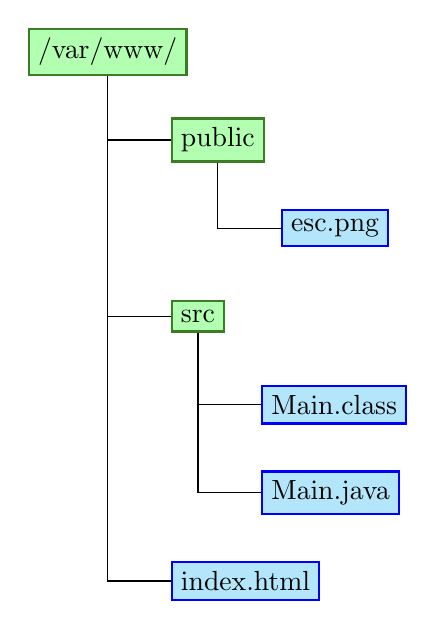
\begin{tikzpicture}[scale=1.6,
    every node/.style = {draw=black, thick, anchor=west},
    selected/.style = {draw=OliveGreen, fill=green!30},
    file/.style = {draw=blue, fill=cyan!30},
    optional/.style = {dashed, fill=gray!50},
    grow via three points={one child at (0.5,-0.7) and two children at (0.5,-0.7) and (0.5,-1.4)},
    edge from parent path={(\tikzparentnode.south) |- (\tikzchildnode.west)}
]
\node [selected] {/var/www/}
    child { node [selected] {public}
        child { node [file] {esc.png}}
        child [missing] {}
    }
    child [missing] {}
    child { node [selected] {src}
        child { node [file] {Main.class}}
        child { node [file] {Main.java}}
    }
    child [missing] {}
    child [missing] {}
    child { node [file] {index.html}};
\end{tikzpicture}
\end{tcolorbox}
\end{minipage}%
\hspace{-1.5cm}
\begin{minipage}[t]{0.6\textwidth}
\vspace{0pt}
Soit l'arborescence à gauche d'un système de fichiers (filesystem).
Écrivez un programme Python (utilisant \texttt{match}) qui affiche \textbf{seulement les noms des fichiers} dans un seul dossier spécifié à la ligne de commande. 
Votre programme doit seulement gérer les arguments suivants: \newline 

\begin{itemize}
    \item[$\bullet$] \texttt{/var/www/./public/..}
    \item[$\bullet$] \texttt{/var/www/src/..}
    \item[$\bullet$] \texttt{/var/www/src/}
    \item[$\bullet$] \texttt{/var/www/public/} \newline 
\end{itemize}

Pour les autres cas, il faut afficher \texttt{La saisie n'était pas reconnue}.  
\end{minipage}
\begin{conseil}
Pour spécifer un argument à la ligne de commande en Python \href{https://docs.python.org/fr/3.13/library/sys.html\#sys.argv}{consultez cette documentation en ligne}. Pour le \texttt{match} en Python, consultez \href{https://moodle.unil.ch/pluginfile.php/3532635/mod_resource/content/5/3\%20\%E2\%80\%93\%20Programming\%20Basics.pdf}{la diapositive 39 du cours}. 
\end{conseil}


\textbf{Re-faire} cet exercice en utilisant \texttt{input} pour lire la saisie de l'utilisateur.
\begin{conseil}
La documentation de \texttt{input} est \href{https://docs.python.org/fr/3.13/library/functions.html\#input}{disponible sur ce lien}.
\end{conseil} 

\begin{solution}
 \lstinputlisting{solutions/question14.py}
\end{solution}

\begin{solution}
 \lstinputlisting{solutions/question14_2.py}
\end{solution}
\end{Exercice}

\section{Type casting}


\begin{Exercice}[5 minutes] \textbf{Conversion des variables (Type casting) (Java ou Python)}\\
   Qu'affichent les programmes suivants ? \\
   
   \textbf{Python:}
   \lstinputlisting{code/question15.py}
   
   \textbf{\\Java:}
   \lstinputlisting{code/Question15.java}
    
   
    \begin{conseil}
      	Attention, ces fonctions ne changent pas le type des variables, elles ne font que les convertir.
        
    \end{conseil}
    \begin{solution}
     
    \textbf{Python:}\\
    3\\
    3.0
    
    \textbf{\\Java:}\\
    3\\
    3.14 \\
    \end{solution}   
\end{Exercice}

\section{Chaîne de caractères}
\begin{Exercice}[10 minutes]

Soit la chaîne de caractères: \texttt{UNIL\textbackslash nSchool\textvisiblespace of\textvisiblespace Criminal\textvisiblespace Sciences}. 

\begin{figure}[ht]

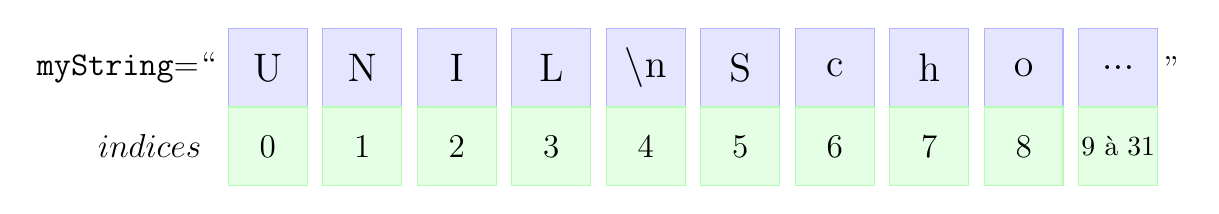
\begin{tikzpicture}[scale=1]
    % Define the string characters
    \def\chars{{"U", "N", "I", "L", "\textbackslash n", "S", "c", "h", "o", "..."}}

    \node at (-1.3, 0.5) {\large \texttt{myString}=``};
    \node at (12, 0.5) {\large ''};
    \node at (-1, -0.5) {\large $indices$};

    
    % Draw cells for each character
    \foreach \i in {0,...,9} {
        % Draw character cell
        \draw[fill=blue!10, draw=blue!30] (\i*1.2, 0) rectangle (\i*1.2+1, 1);
        \node at (\i*1.2+0.5, 0.5) {\Large\pgfmathparse{\chars[\i]}\pgfmathresult};
        
        % Draw index cell
        \draw[fill=green!10, draw=green!30] (\i*1.2, -1) rectangle (\i*1.2+1, 0);
        \ifnum\i=9
            \node at (\i*1.2+0.5, -0.5) {9 à 31};
        \else
            \node at (\i*1.2+0.5, -0.5) {\large\i};
        \fi
    }
    
    % Add labels
    % \node[above] at (5.4, 1.2) {\textbf{Caractères}};
    % \node[below] at (5.4, -1.2) {\textbf{Indices}};
\end{tikzpicture}

\end{figure}

\begin{attention}
Ici, le caractère \textvisiblespace \ est seulement pour mettre en évidence le caractère espace. 
\end{attention}
\begin{enumerate}
\item Affichez cette chaîne en Python et en Java. Pourquoi est-elle séparée par une nouvelle ligne?
\item Essayez d'afficher uniquement la chaîne \texttt{School of Crimi} en sélectionnant une sous-chaîne de la chaîne initiale. 
\begin{conseil}
    \begin{itemize}
        \item Pour créer une sous-chaîne en Java, utilisez la méthode \texttt{myString.substring(int beginIndex, int endIndex)} où \texttt{beginIndex} est l'indice du premier caractére dans la chaîne \texttt{myString} que l'on veut inclure dans la sous-chaîne et \texttt{endIndex} est l'indice du caractère suivant le dernier à inclure (le caractère à l'indice \texttt{endIndex} n'est pas inclus dans la sous-chaîne).
        \item Pour créer une sous-chaîne en Python, utilisez l'opérateur slice \texttt{myString[beginIndex, endIndex]} et pareil pour l'interprétation du \texttt{beginIndex}, \texttt{endIndex}, et \texttt{myString}.
    \end{itemize}
\end{conseil}
\item Affichez le troisième caractère de la chaîne en Python et en Java. 
\begin{conseil}
    \begin{itemize}
        \item Pour obtenir le $i$eme caractère en Java, on écrit \texttt{myString.charAt(i)}.
    \item Pour obtenir le $i$eme caractère en Python, on écrit \texttt{myString[i]}.
    \end{itemize}
\end{conseil}
\item Imprimer la longueur de la chaîne en Python et en Java.
\begin{conseil}
    Utiliser la méthode \texttt{myString.length()} en Java et la fonction \texttt{len} en Python.
\end{conseil}
\end{enumerate}
\begin{solution}
    Pour la question 1, la ligne est separée à cause du charactère \lstinline{\\n} qui crée un saut de ligne.
\end{solution}
\begin{solution}
   \lstinputlisting{solutions/question16.py}
\end{solution}
\begin{solution}
   \lstinputlisting{solutions/Question16.java}
\end{solution}
\end{Exercice}

\end{document}
